
\tikzstyle{group} = [draw=red,ultra thick]

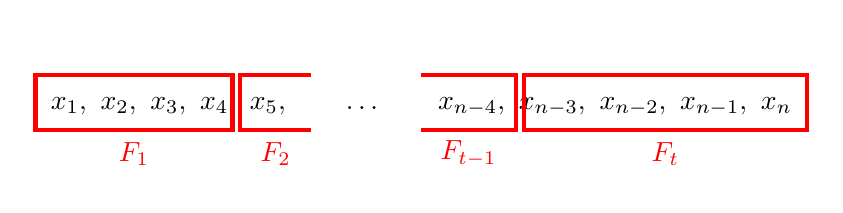
\begin{tikzpicture}
    \path (-5, -1) -- (5, -1) -- (5, 1) -- (-5, 1) -- cycle;
    \node[] at (0,0) {$x_1,\ x_2,\ x_3,\ x_4,\ x_5, \qquad \dots \qquad x_{n-4},\ x_{n-3},\ x_{n-2},\ x_{n-1},\ x_n$};

    \draw<4-> [style=group] (-4.9,-.3) -- (-2.4,-.3) -- (-2.4, .4) -- (-4.9, .4) -- cycle;
    \draw<4-> [style=group] (-1.4, .4) -- (-2.3, .4) -- (-2.3,-.3) -- (-1.4,-.3);
    \draw<4-> [style=group] (0, .4) -- (1.2, .4) -- (1.2,-.3) -- (0,-.3);
    \draw<4-> [style=group] (4.9, -.3) -- (1.3,-.3) -- (1.3, .4) -- (4.9, .4) -- cycle;

    \node<4-> at (-3.65, -.6) {\color{red}$F_1$};
    \node<4-> at (-1.85, -.6) {\color{red}$F_2$};
    \node<4-> at (.6, -.6) {\color{red}$F_{t-1}$};
    \node<4-> at (3.1, -.6) {\color{red}$F_t$};
\end{tikzpicture}